\newcommand{\annotKasiski}[4]{\textcolor{#1}{\(\underset{\text{\tiny #4}}{\texttt{#2}}\)#3}}

\begin{frame}[fragile]{Häufigkeiten Bi- und Trigramme}
%\resizebox{\textwidth}{!}{
\begin{table}[H]
  \centering
  \tiny
  \begin{subtable}[t]{0.32\textwidth}
  \centering
  \begin{tabular}{c|p{1.5cm}}
  \textbf{Buchstabe} & \textbf{Relative\newline Häufigkeit (\%)} \\ \midrule
  E & 17.40 \\ \midrule
  N & 9.78 \\ \midrule
  I & 7.55 \\ \midrule
  S & 7.27 \\ \midrule
  R & 7.00 \\ \midrule
  ... & ... \\ 
  \end{tabular}
  \caption{Buchstabenhäufigkeit}
  \label{tab:buchstaben-haeufigkeit}
  \end{subtable}
  \begin{subtable}[t]{0.32\textwidth}
  \centering
  \begin{tabular}{c|p{1.5cm}}
  \textbf{Bigramm} & \textbf{Relative\newline Häufigkeit (\%)} \\ \midrule
  ER & 3.94 \\ \midrule
  EN & 3.07 \\ \midrule
  CH & 2.73 \\ \midrule
  DE & 2.41 \\ \midrule
  EI & 2.29 \\ \midrule
  ... & ... \\ 
  \end{tabular}
  \caption{Bigrammhäufigkeit}
  \label{tab:bigramme-haeufigkeit}
  \end{subtable}
  \begin{subtable}[t]{0.32\textwidth}
  \centering
  \begin{tabular}{c|p{1.5cm}}
  \textbf{Trigramm} & \textbf{Relative\newline Häufigkeit (\%)} \\ \midrule
  DER & 1.44 \\ \midrule
  SCH & 1.21 \\ \midrule
  ICH & 1.08 \\ \midrule
  DIE & 0.98 \\ \midrule
  UND & 0.95 \\ \midrule
  ... & ... \\ 
  \end{tabular}
  \caption{Trigrammhäufigkeit}
  \label{tab:trigramme-haeufigkeit}
  \end{subtable}
%  \caption{Relative Häufigkeiten der Buchstaben, Bigramme und Trigramme im Deutschen}
%  \label{tab:alle-haeufigkeiten}
  \end{table}
%}
\end{frame}


\begin{frame}[fragile, label=kasiski]{Angriff auf Vigenère: Unbekannte Schlüssellänge}{\textbf{Kasiski-Test}}

\texttt{W\red{EIN}SCH\red{EIN}TMIRF\red{EIN}ZUS\red{EIN}\\
C\red{ODE}COD\green{ODE}DECOD\green{ODE}DEC\red{ODE}\\
Y\annotKasiski{red}{S}{LR}{2}UQK\annotKasiski{ForestGreen}{I}{KB}{8}WQKFI\annotKasiski{ForestGreen}{I}{KB}{16}CYU\annotKasiski{red}{S}{LR}{22}}\\[1cm]

\begin{itemize}
    \item \enquote{\red{SLR}} und \enquote{\green{IKB}} kommen je zweimal im Geheimtext vor
    \item Distanz zwischen Positionen = Vielfaches der Schlüssellänge?
    \begin{itemize}
    \item \texttt{SLR}: Positionen 2 und 22. $\rightarrow$ 22-2 = 20 = $\red{2\times 2} \times 5$\only<2->{\\
        $\mathbf{\underset{\text{Position 1 \texttt{SLR}}}{2}+\underset{\text{Codewort-Länge!}}{4}\times \underset{\text{Anzahl Codewörter}}{5} = \underset{\text{Position 2 \texttt{SLR}}}{22}}$}
    \item \texttt{IKB}: Positionen 8 und 16. $\rightarrow$ 16-8 = 8  = $\red{2\times 2}\times 2$\only<2->{\\
        $\mathbf{\underset{\text{Position 1 \texttt{IKB}}}{8}+\underset{\text{Codewort-Länge!}}{4}\times \underset{\text{Anzahl Codewörter}}{2} = \underset{\text{Position 2 \texttt{IKB}}}{16}}$}
    \end{itemize}
\end{itemize}
\end{frame}
\begin{frame}[label=kasiski2]{Angriff auf Vigenère: \textbf{Kasiski-Test}}
\only<1>{
Angenommen, wir haben folgenden Text, verschlüsselt mit dem Wort ``BALMER'':
\begin{figure}[H]
        \centering
        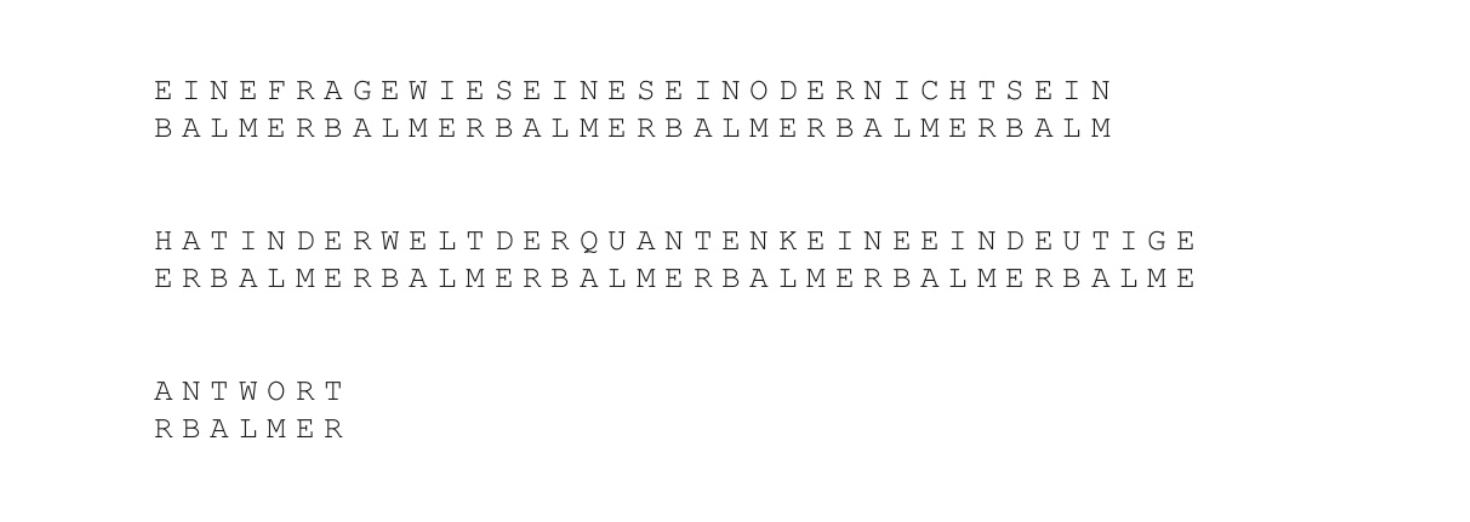
\includegraphics[width=\textwidth]{GrundlagenInfo/03_Kryptologie/Figures/Kasiski1.png}
\end{figure}
}
\only<2>{
Wir suchen nun zuerst im Geheimtext nach Trigrammen, die mehrmals vorkommen:
\begin{figure}[H]
        \centering
        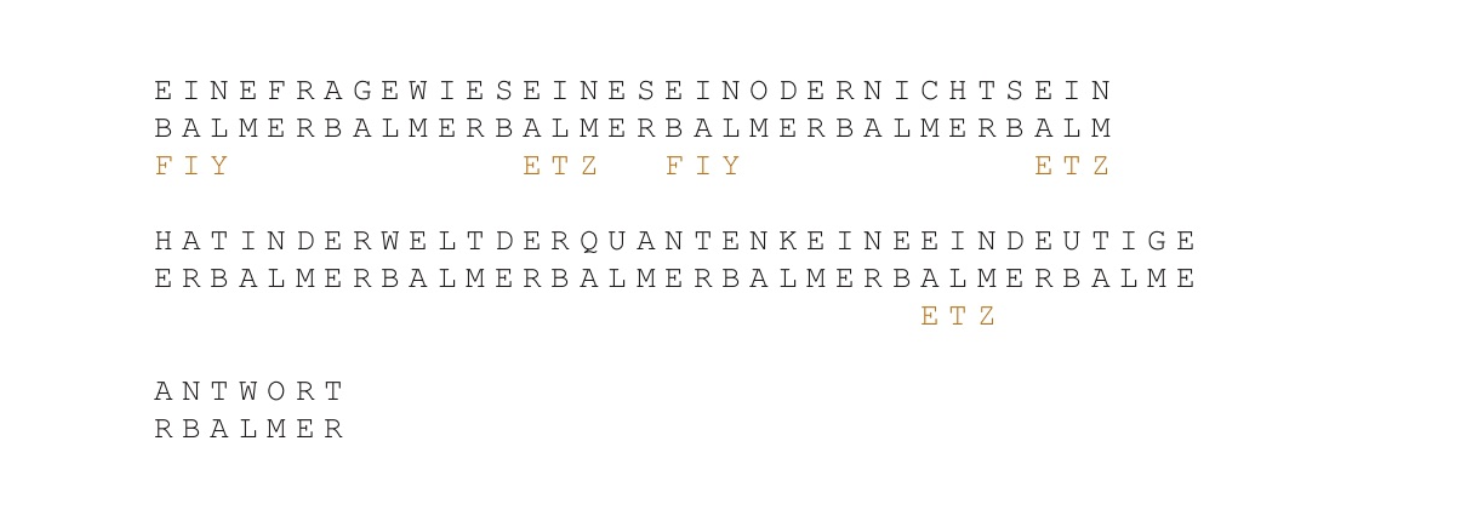
\includegraphics[width=\textwidth]{GrundlagenInfo/03_Kryptologie/Figures/Kasiski2.png}
\end{figure}
}
\only<3>{
Wir notieren die Anfangs-Positionen der Trigramme:
\begin{figure}[H]
        \centering
        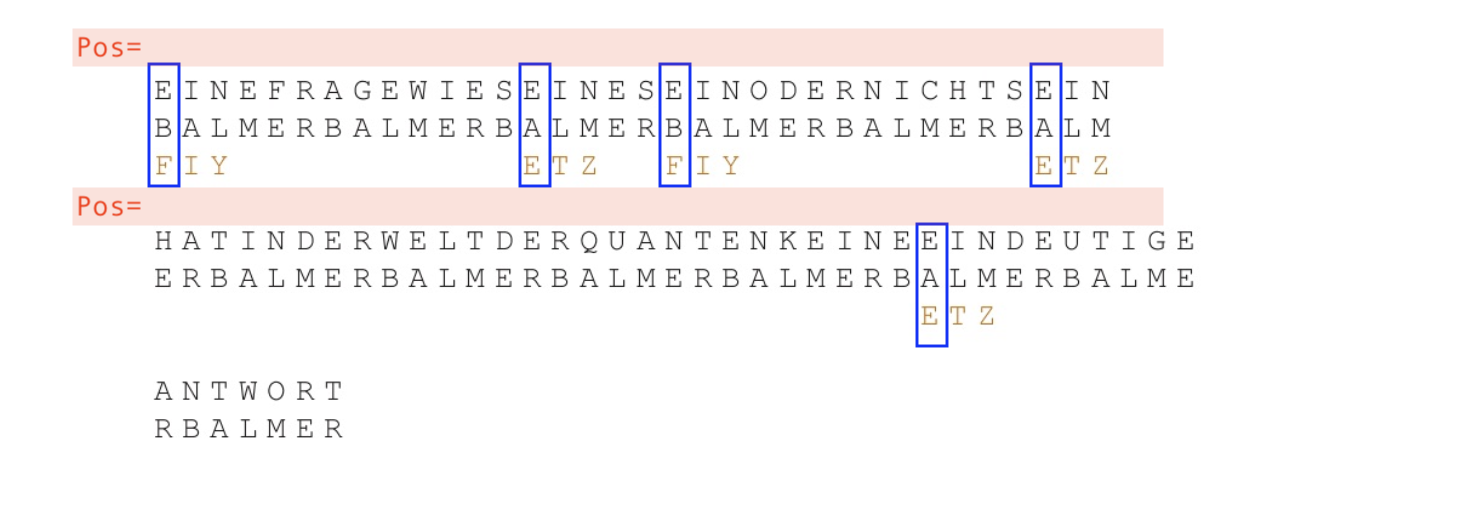
\includegraphics[width=\textwidth]{GrundlagenInfo/03_Kryptologie/Figures/Kasiski3.png}
\end{figure}
}
\only<4->{
Wir notieren die Anfangs-Positionen der Trigramme:
\begin{figure}[H]
        \centering
        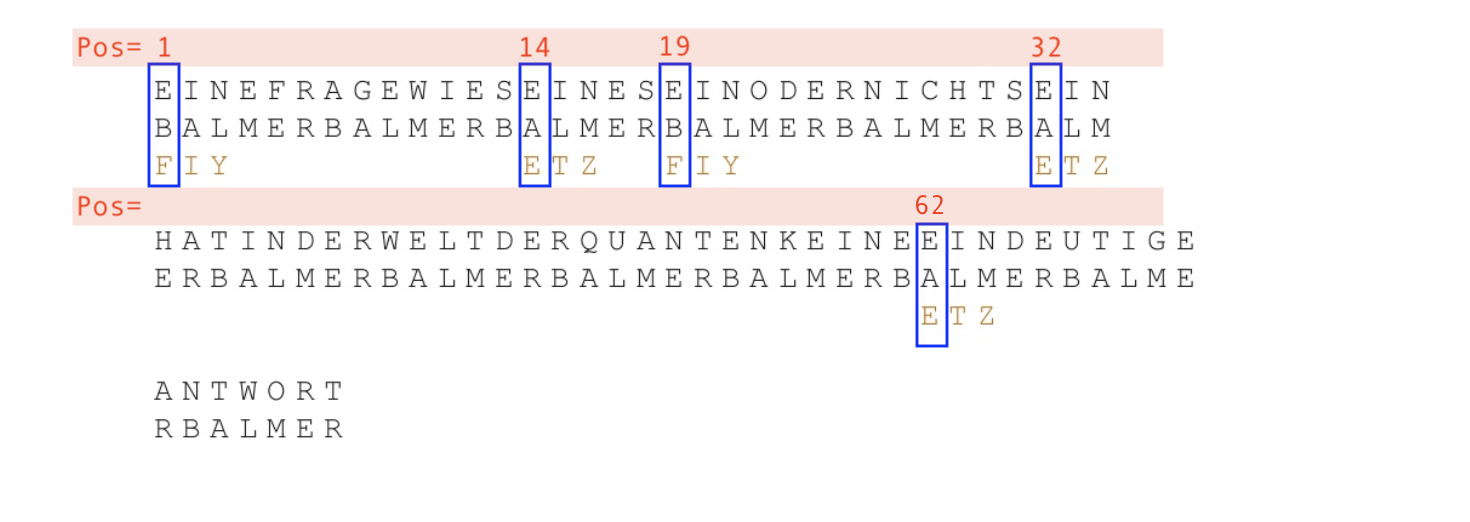
\includegraphics[width=\textwidth]{GrundlagenInfo/03_Kryptologie/Figures/Kasiski4.png}
\end{figure}
}
\only<5->{
Nun können wir die Abstände zwischen den mehrfach vorkommenden Trigrammen berechnen:
\begin{align*}
62 - 14 = 48 = 2^4\cdot 3\\
62 - 32 = 30 = 2 \cdot 3 \cdot 5\\
32 - 14 = 18 = 2 \cdot 3^2
\end{align*}
GGT = 6 $\rightarrow$ Länge des Schlüsselworts.
}
\end{frame}

\begin{frame}[fragile]{Auftrag}
\begin{center}
\aufgabebox{Arbeitsblatt, Aufgabe 1.3}
\end{center}
\end{frame}